Figure \ref{fig:img2_src} shows the original image, which is filled with black and white pixels. This kind of noise is known as salt--and--pepper noise, and from the histogram of the image (figure \ref{fig:img2_hist}) can the amount of salt--and--pepper noise be seen; salt noise on the right and pepper noise on the left. 
\begin{figure}[H]
    \centering
    \begin{subfigure}[b]{0.23\textwidth}
        \includegraphics[width=\textwidth]{img2/src.png}
        \caption{The original image}
        \label{fig:img2_src}
    \end{subfigure}
    \begin{subfigure}[b]{0.446\textwidth}
        \includegraphics[width=\textwidth]{img2/hist.png}
        \caption{Histogram of the original image}
        \label{fig:img2_hist}
    \end{subfigure}
    \caption{Analysis of image 2}\label{fig:img2}
\end{figure}

Approximately  there are three times more salt noise compared to the pepper noise. The values in the middle of the histogram is what is left of the original image, and in order to restore as much as possible, and median filter is applied on the image. \todo{How do we know.. det kunne også være en form for noise, vi ved kun med sikkerhed at pepper of salt er tydeligt. hvilket kan ses og bekræftes via hist. }The median filter is chosen because it is very effective against salt-and-pepper noise in the images, and the OpenCV function
\begin{center}
\lstinline|void medianBlur(InputArray src, OutputArray dst, int ksize)|\footnote{\url{http://docs.opencv.org/2.4/modules/imgproc/doc/filtering.html\#void medianBlur(InputArray src, OutputArray dst, int ksize)}}
\end{center}
is used for applying this filter to the image. The median filter help blurring the image, and depending on the size of \lstinline|ksize|, the more blurred will the image become.\\[0.2cm]
The \lstinline|ksize| is the size of the kernel filter applied to each pixel in the image, and therefore must the value of \lstinline|ksize| be odd and greater than 1, so in order to test if the noise is removed, a kernel of \lstinline|3| is applied on the image 2 and checked if all the noise is removed. If not all the noise is removed, the kernel size is increased with two, and checked again, and so on.  

\begin{figure}[H]
    \centering
    \begin{subfigure}[b]{0.24\textwidth}
        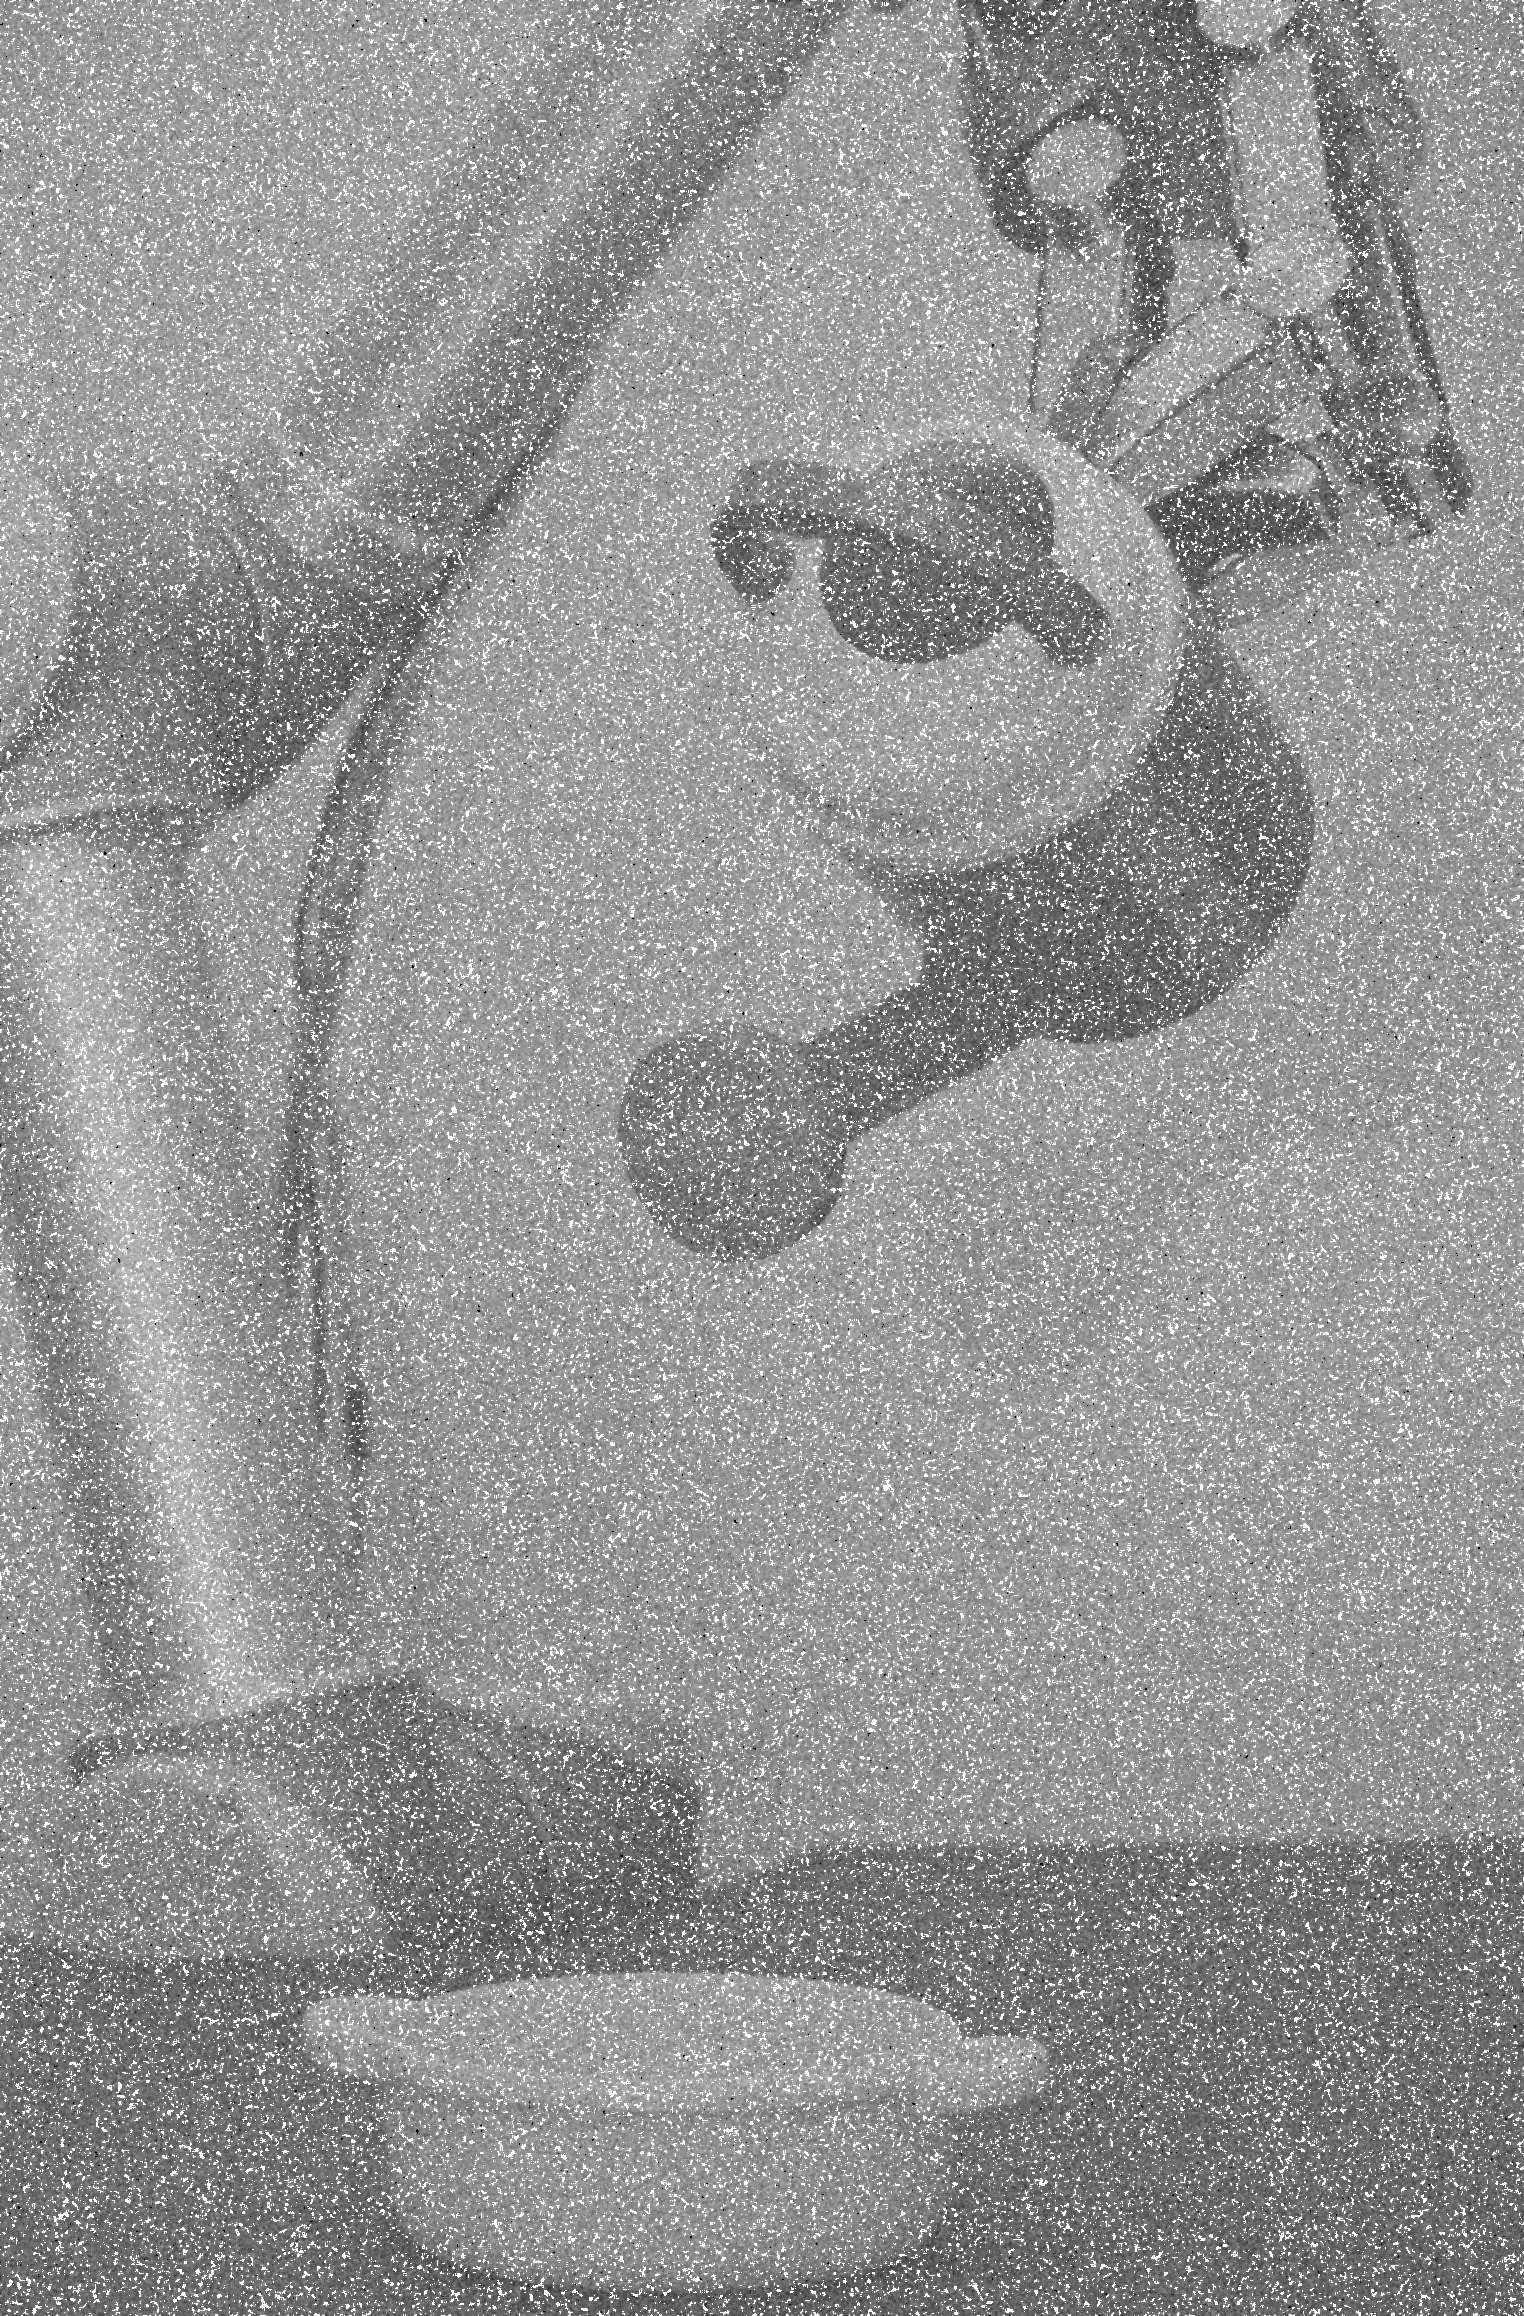
\includegraphics[width=\textwidth]{img2/median3.png}\\[0.1cm]
        \includegraphics[width=\textwidth]{img2/kernel3.png}
        \caption{\lstinline|ksize = 3|}
        \label{fig:img2_kernel3}
    \end{subfigure}
    \begin{subfigure}[b]{0.24\textwidth}
        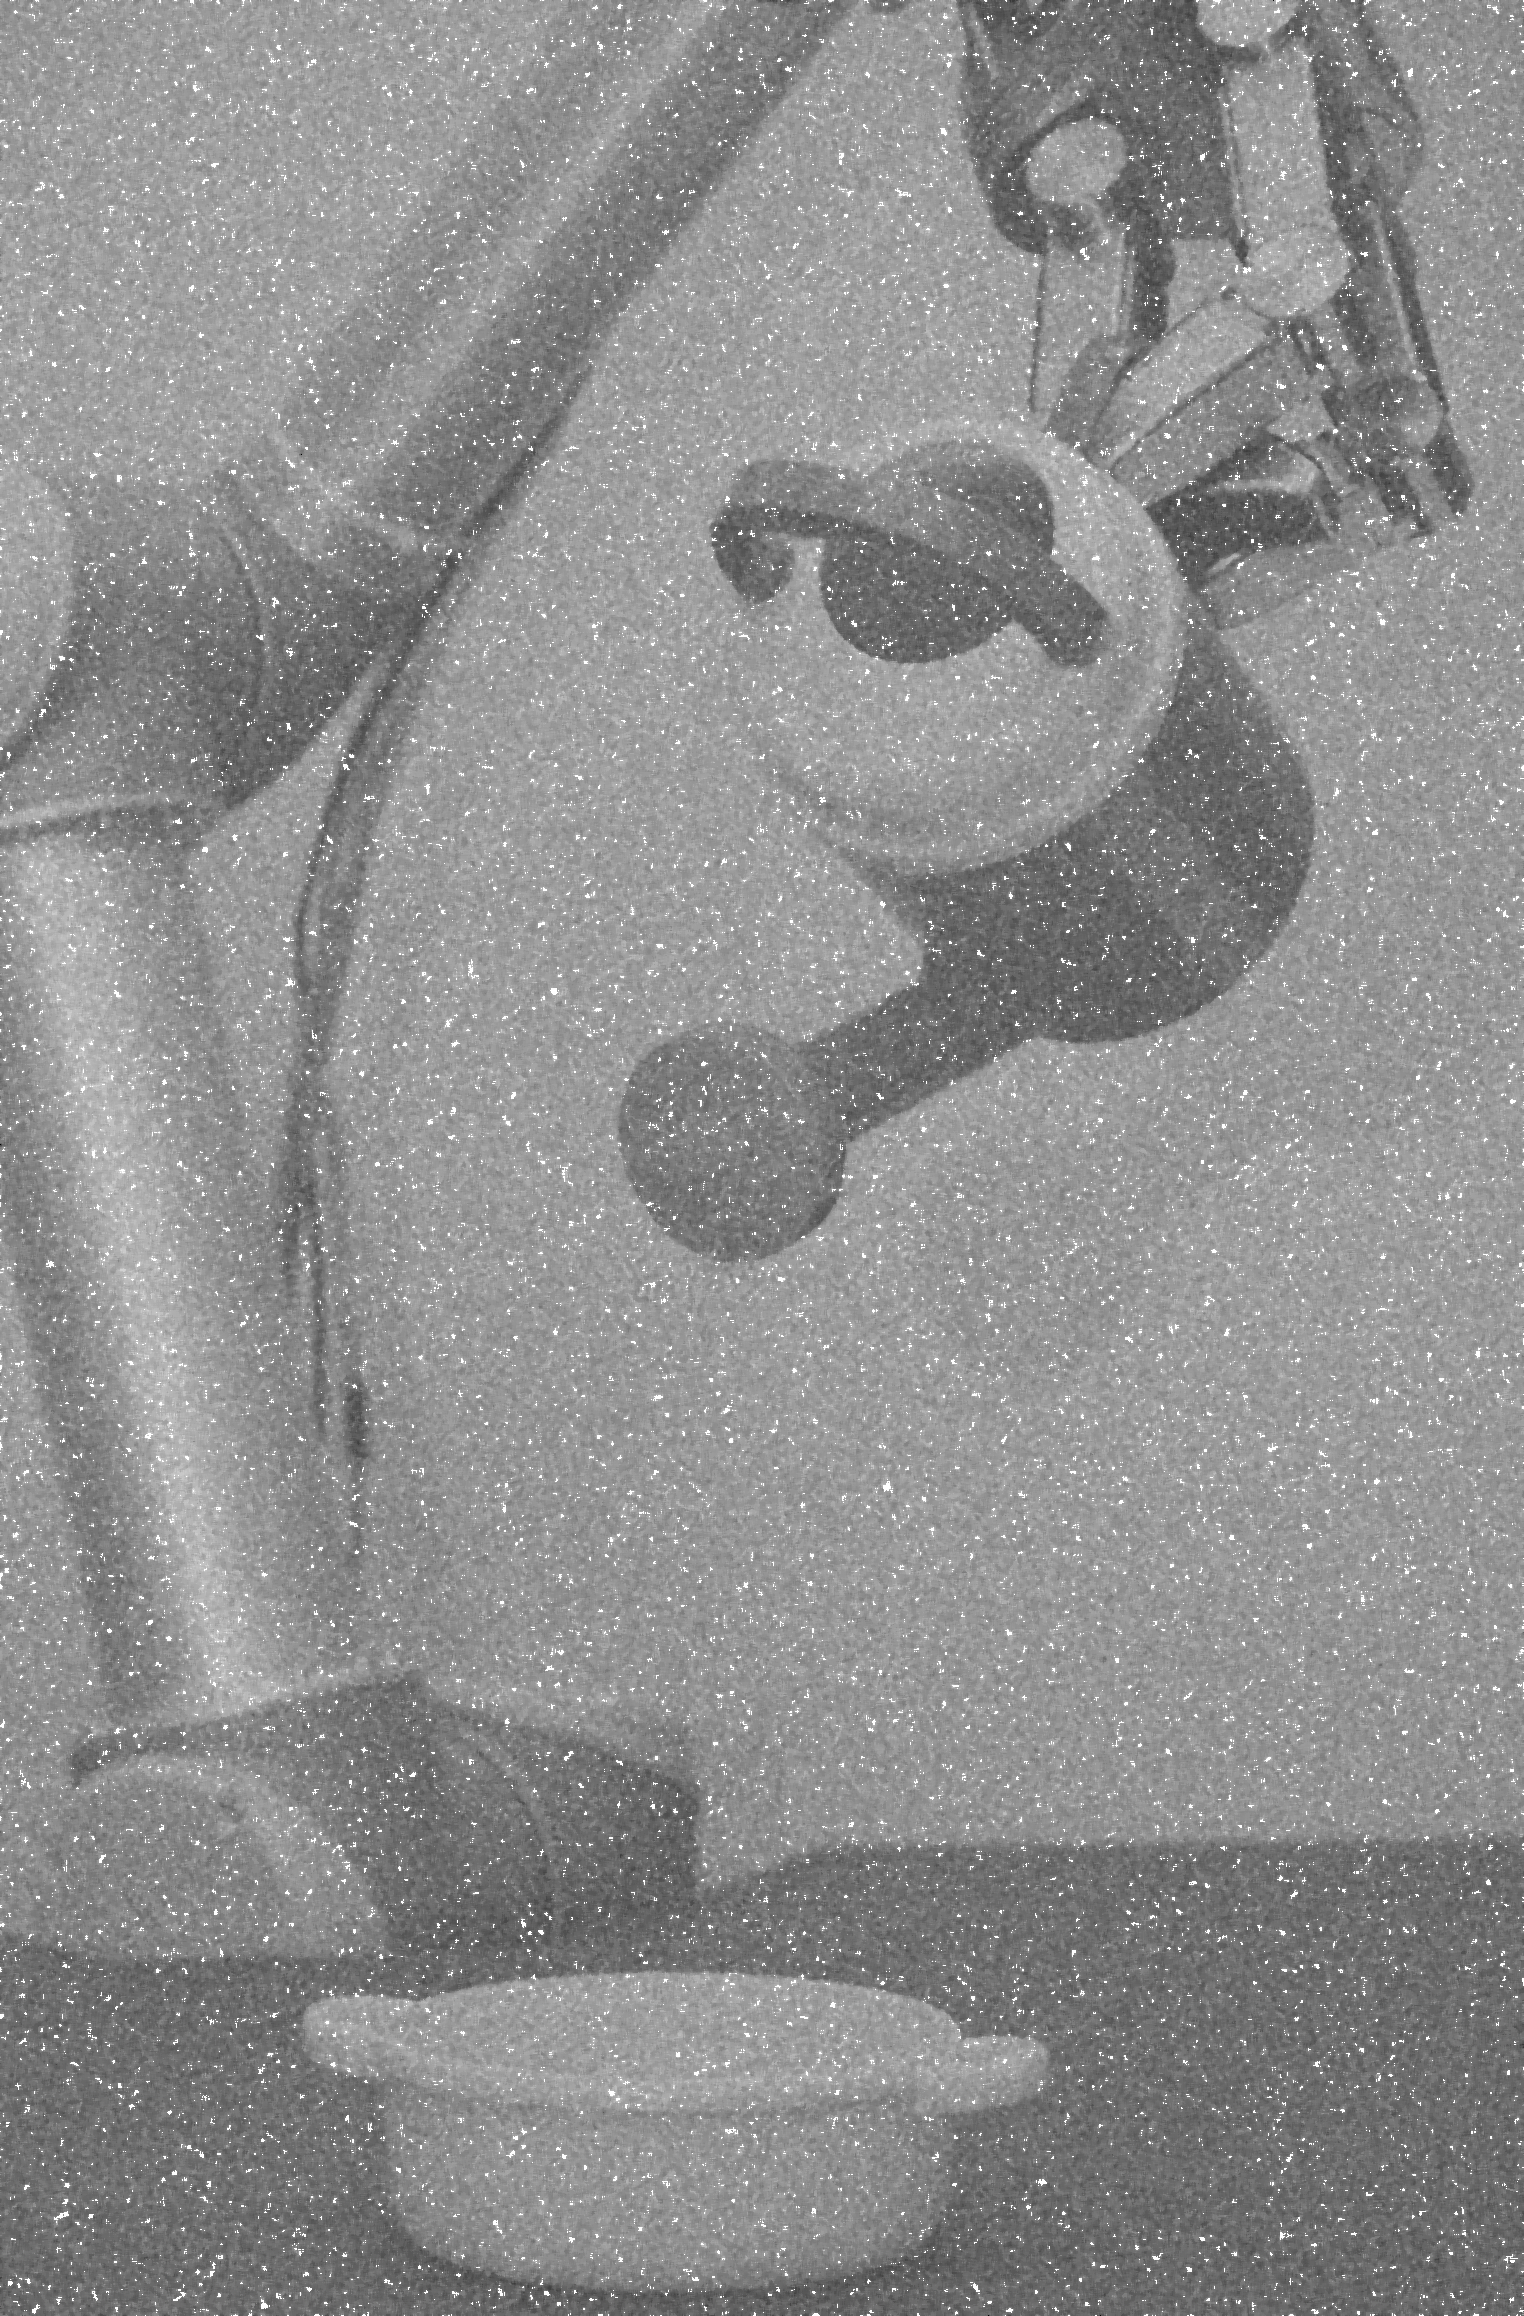
\includegraphics[width=\textwidth]{img2/median5.png}\\[0.1cm]
        \includegraphics[width=\textwidth]{img2/kernel5.png}
        \caption{\lstinline|ksize = 5|}
        \label{fig:img2_kernel5}
    \end{subfigure}
    \begin{subfigure}[b]{0.24\textwidth}
        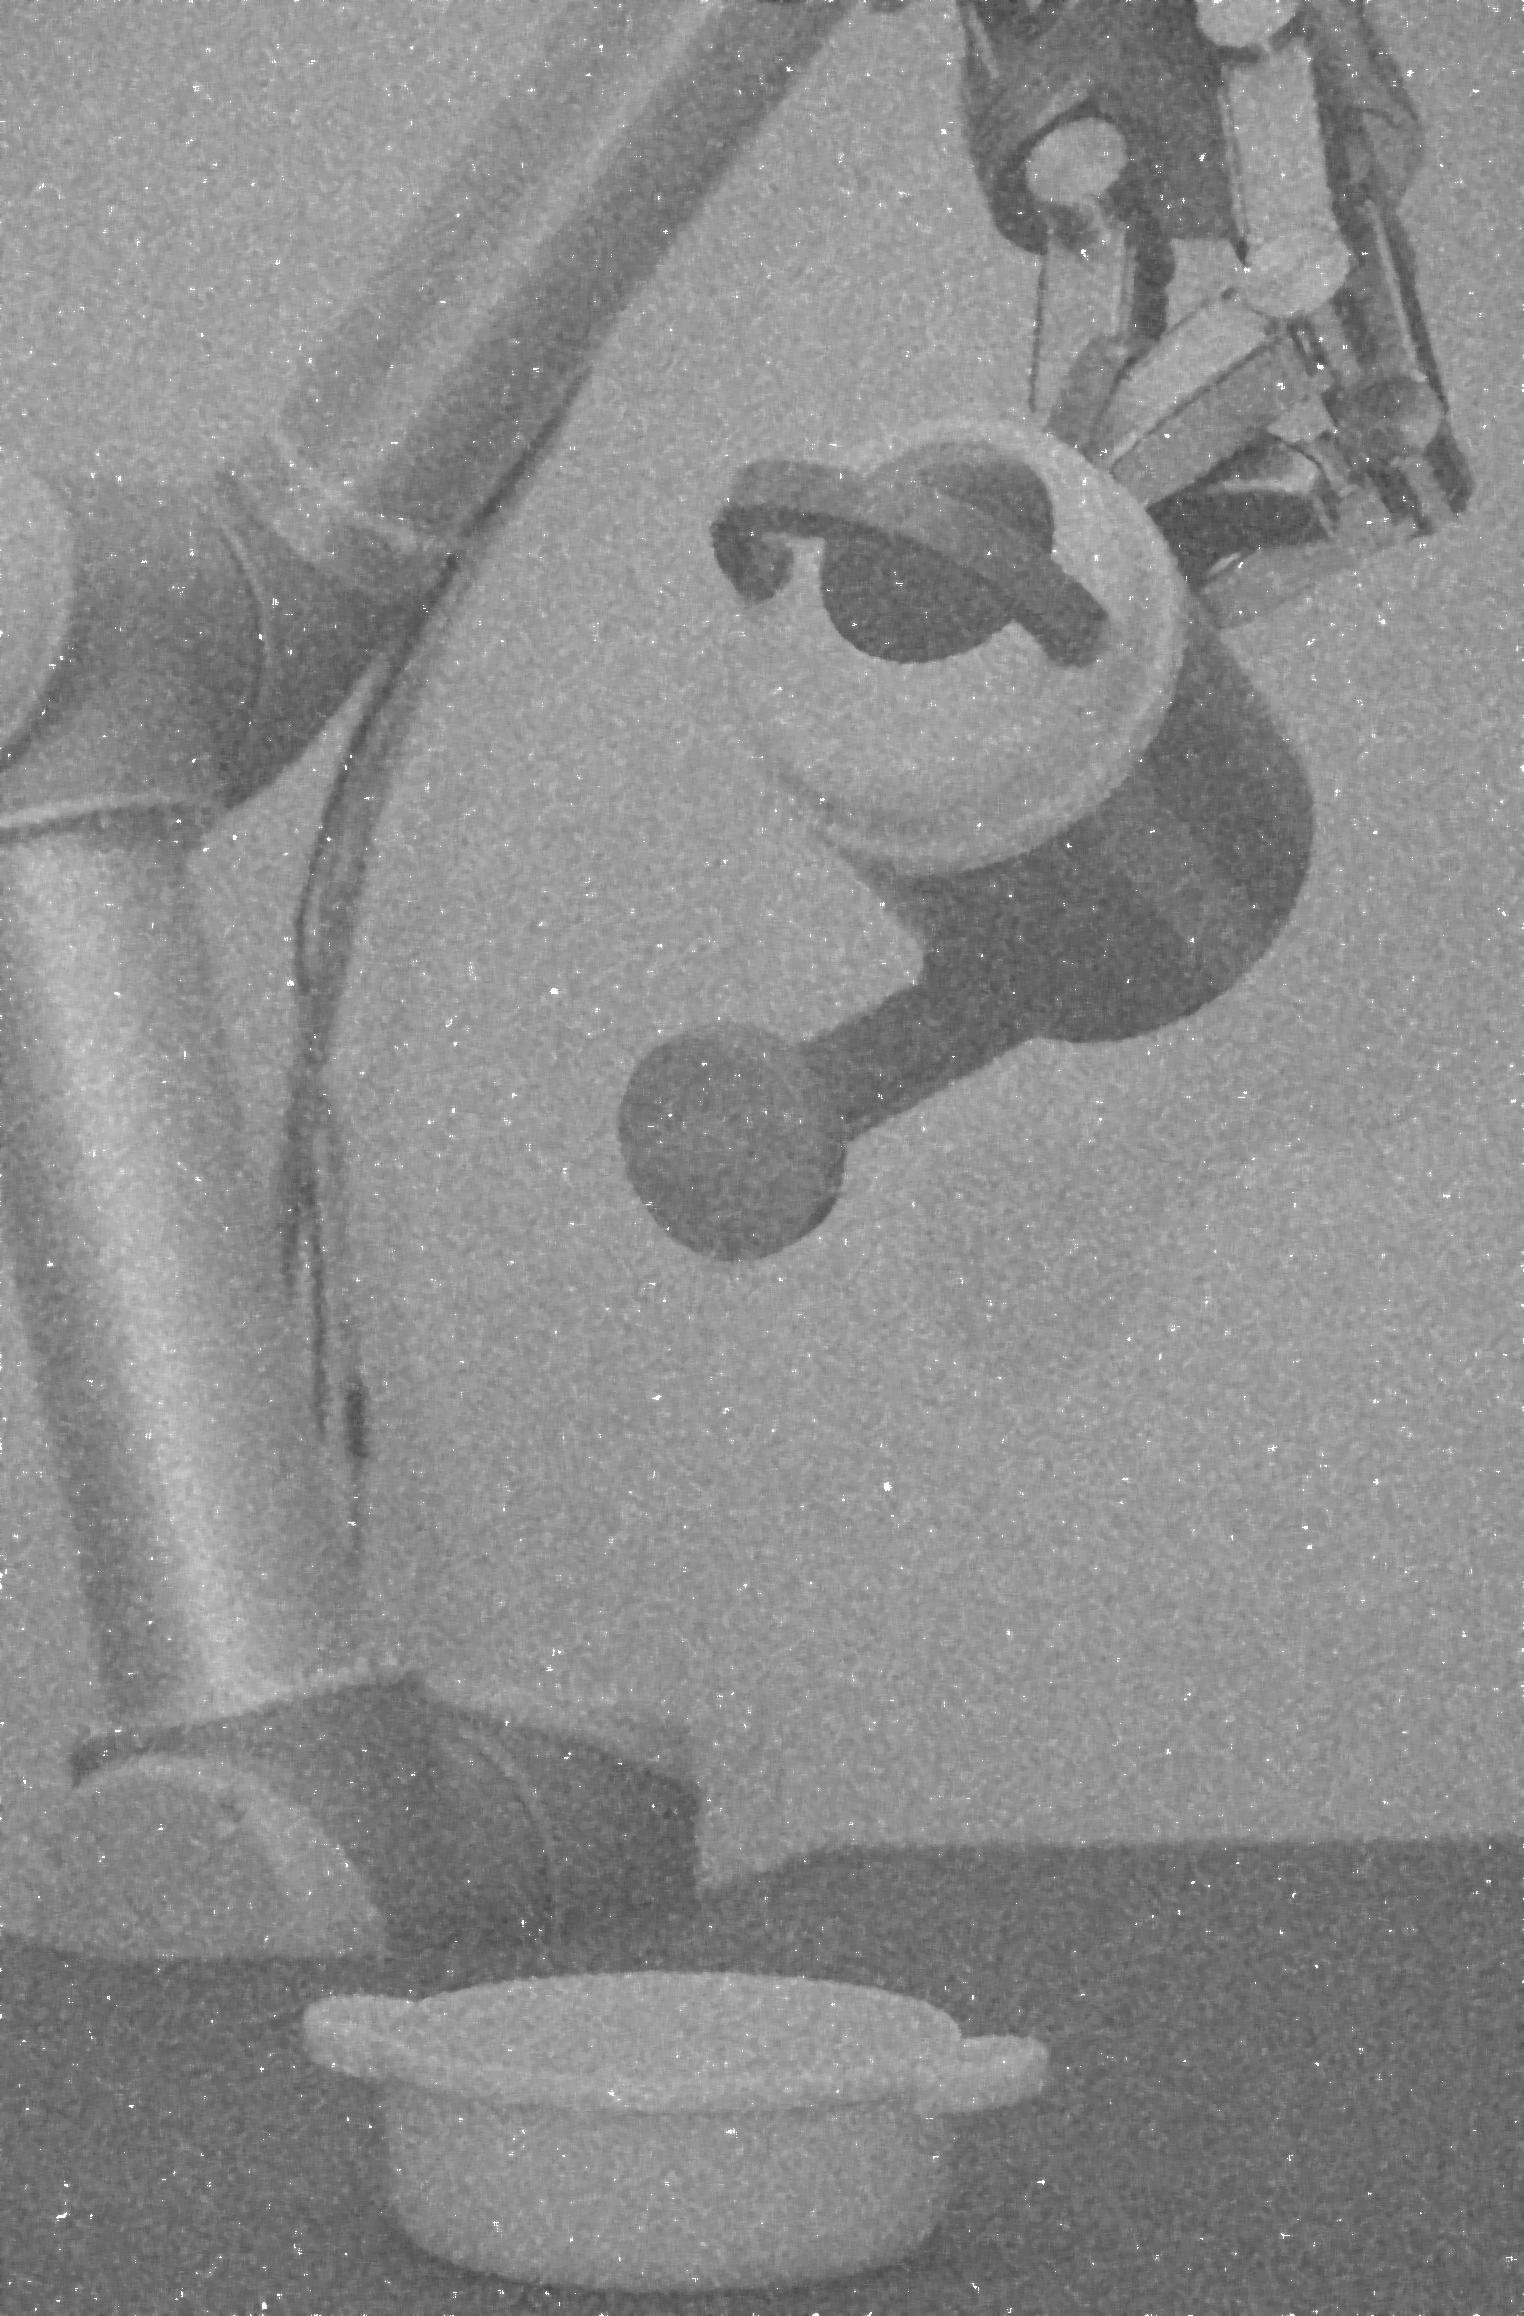
\includegraphics[width=\textwidth]{img2/median7.png}\\[0.1cm]
        \includegraphics[width=\textwidth]{img2/kernel7.png}
        \caption{\lstinline|ksize = 7|}
        \label{fig:img2_kernel7}
    \end{subfigure}
    \begin{subfigure}[b]{0.24\textwidth}
        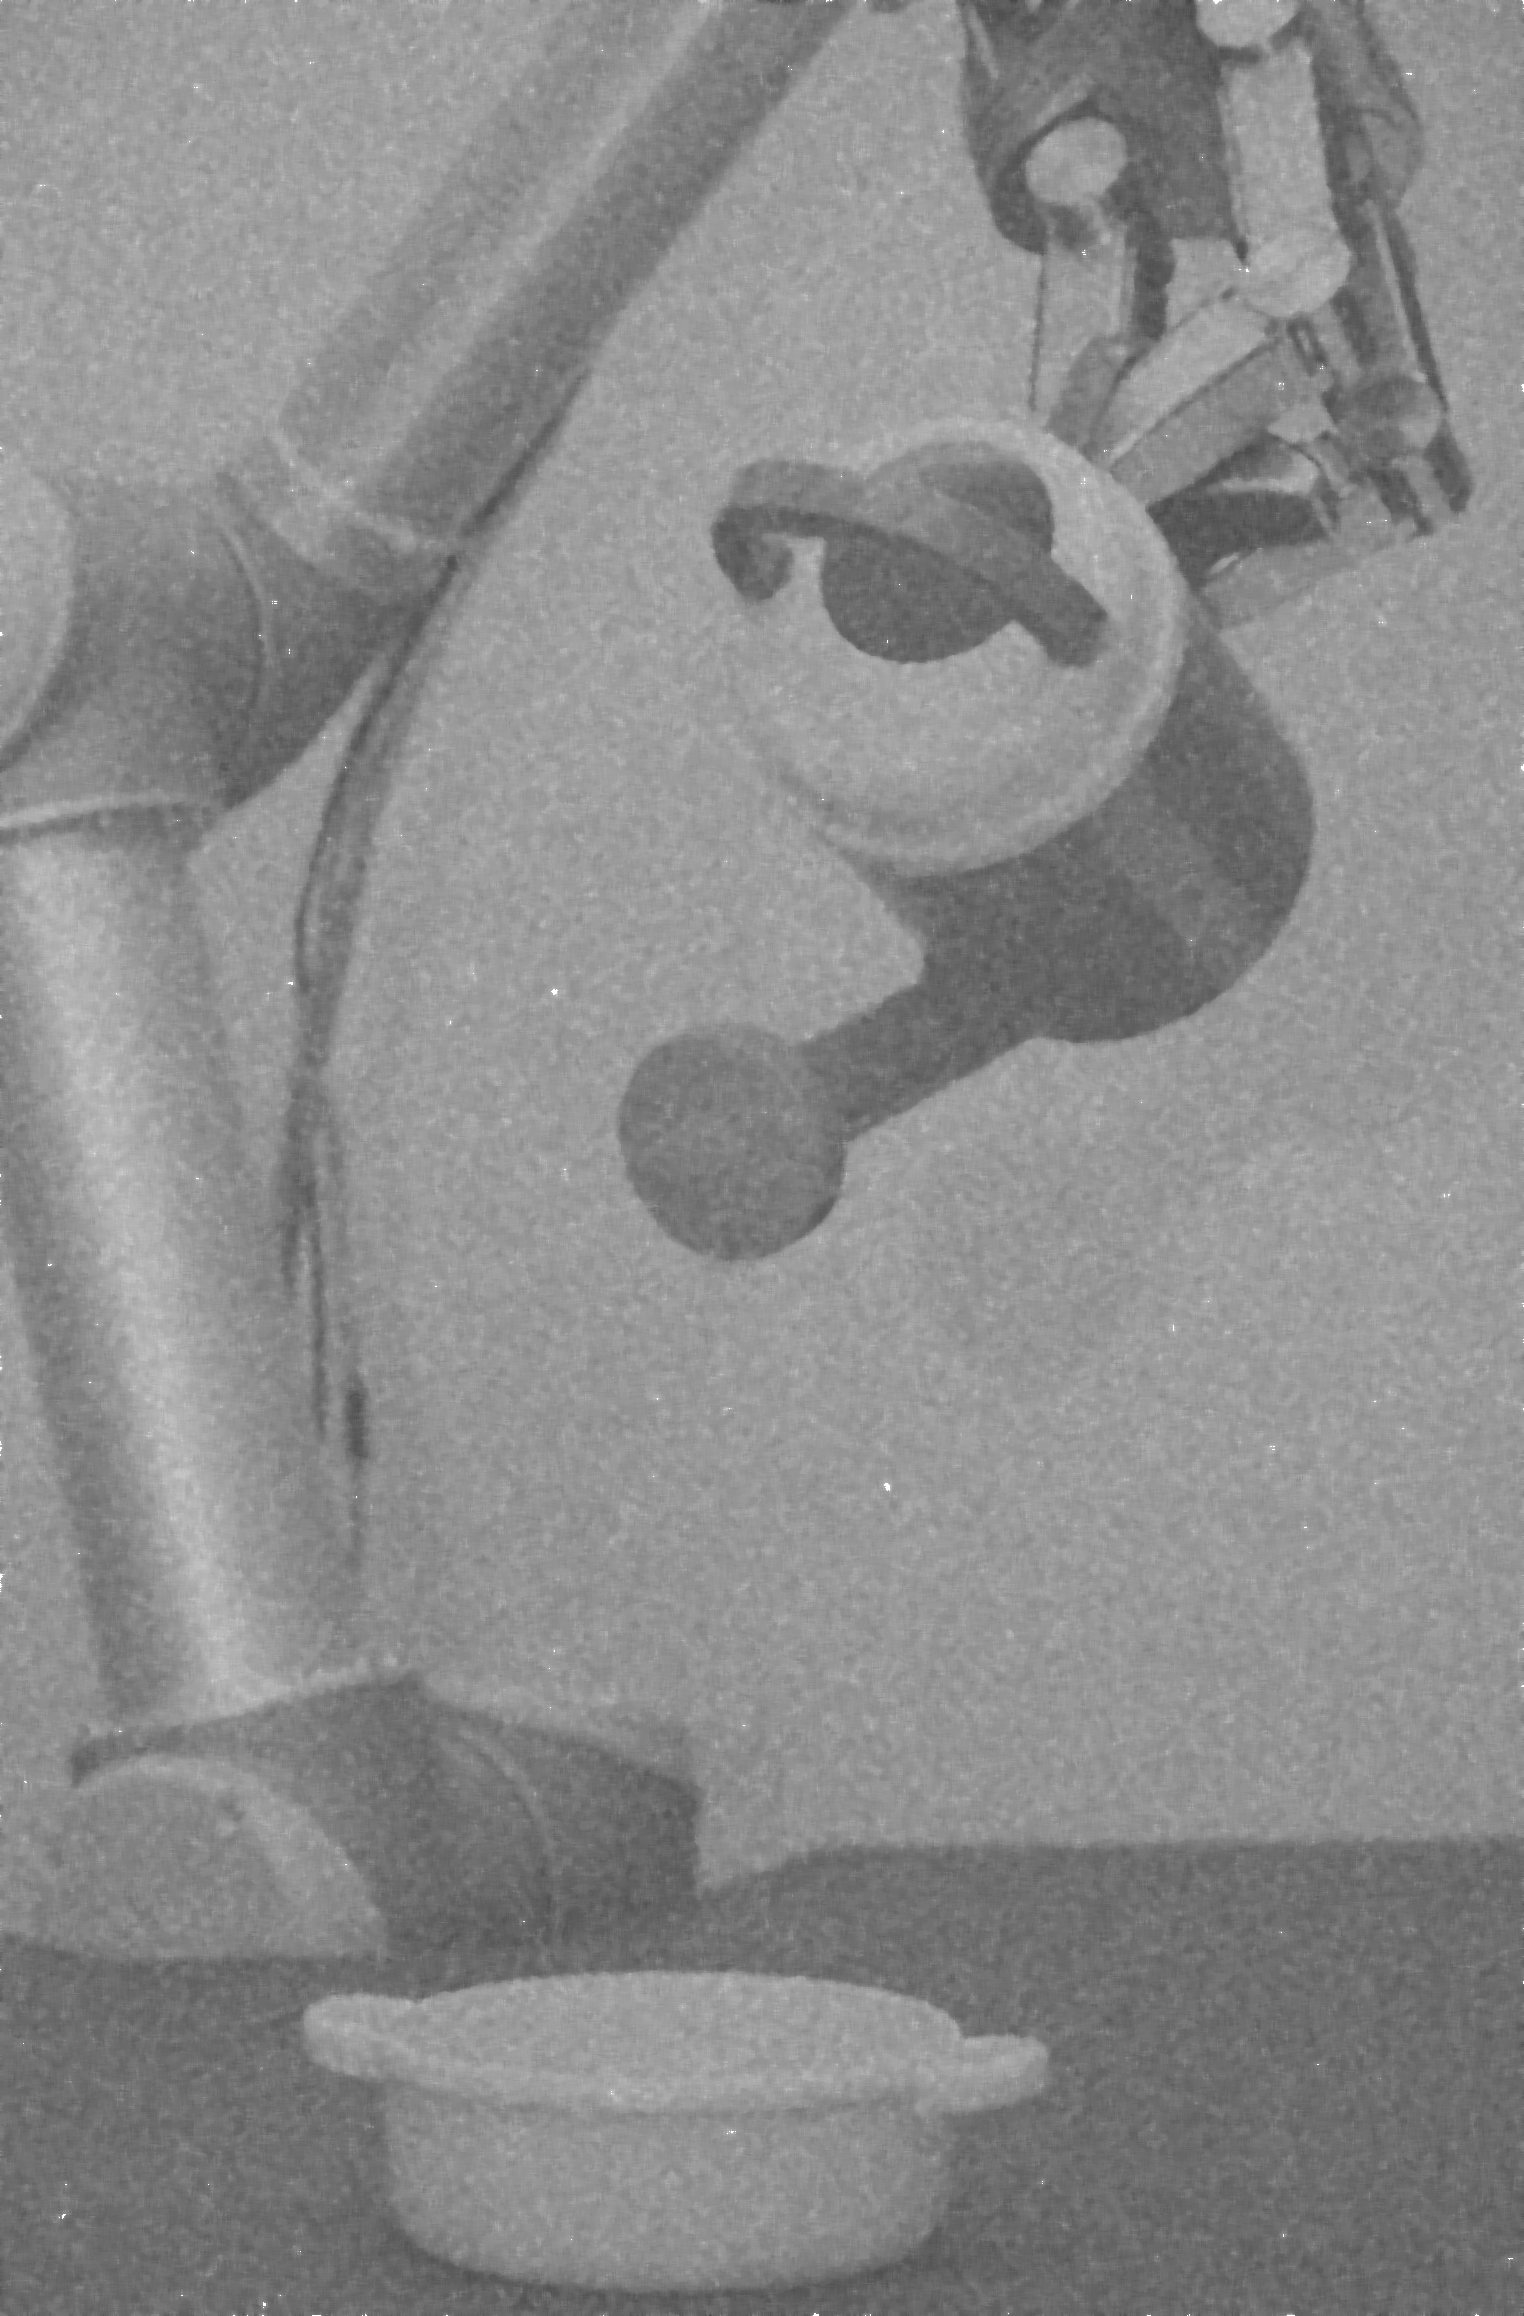
\includegraphics[width=\textwidth]{img2/median9.png}\\[0.1cm]
        \includegraphics[width=\textwidth]{img2/kernel9.png}
        \caption{\lstinline|ksize = 9|}
        \label{fig:img2_kernel9}
    \end{subfigure}
    \caption{Analysis of image 2}\label{fig:img2}
\end{figure}
Figure \ref{fig:img2_kernel3}, \ref{fig:img2_kernel5}, \ref{fig:img2_kernel7} and \ref{fig:img2_kernel9} shows the process of finding the right \lstinline|ksize|, but all four kernel sizes still does not remove all the noise, especially the salt noise. All the salt--and--pepper noise is removed with a \lstinline|ksize=11|, but the disadvantage of this approach is that the details in the image are reduced. For restoring as much as possible of the these details, a histogram equalization is applied on the noise reduced image. Histogram equalization restores the details by improves the contrast in the image by stretching out the intensity range of the image. On the left and right side of image \ref{fig:img2_kernel11}'s histogram are there underpopulated intensities, which is why an histogram equalization is an optimal choice. The result is shown on figure \ref{fig:img2_histEq}.
\begin{figure}[H]
    \centering
    \begin{subfigure}[b]{0.3\textwidth}
        \includegraphics[width=\textwidth]{img2/median.png}\\[0.1cm]
        \includegraphics[width=\textwidth]{img2/histn.png}
        \caption{\lstinline|ksize = 11|}
        \label{fig:img2_kernel11}
    \end{subfigure}
    \begin{subfigure}[b]{0.3\textwidth}
        \includegraphics[width=\textwidth]{org.png}\\[0.1cm]
        \includegraphics[width=\textwidth]{histOrg.png}
        \caption{Equalized}
        \label{fig:img2_org}
    \end{subfigure}
    \begin{subfigure}[b]{0.3\textwidth}
        \includegraphics[width=\textwidth]{img2/eqlMedian.png}\\[0.1cm]
        \includegraphics[width=\textwidth]{img2/histE.png}
        \caption{Equalized}
        \label{fig:img2_histEq}
    \end{subfigure}
    \caption{Analysis of image 2}\label{fig:img2}
\end{figure}
\todo[inline]{Which one is best? -- conclusion needed.. Try contrast streching.. fremfor equalization}